\section{Regno degli Alisei}\label{regno-degli-alisei}

Tags: Stato Creatore: Lorenzo

\section{Regno degli Alisei}\label{regno-degli-alisei-1}

\begin{center}\rule{0.5\linewidth}{0.5pt}\end{center}

\begin{figure}
\centering
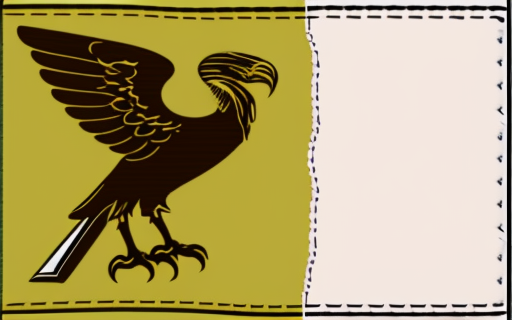
\includegraphics{flag_(1).png}
\caption{flag (1).png}
\end{figure}

Informazioni Generali

Nome Ufficiale: Alisgan

Lingue Ufficiali: Aliseo, Comune Valtarese

Capitale: Dira Mare

Forma di Governo: Repubblica

Popolazione:

Superficie:

Continente: Valtara

Alleati: Rotrekia

\begin{center}\rule{0.5\linewidth}{0.5pt}\end{center}

\subsection{1. Descrizione Generale}\label{descrizione-generale}

\begin{center}\rule{0.5\linewidth}{0.5pt}\end{center}

Il Regno degli Alisei, noto anche come ``Alisgan'' nella lingua madre,
rappresenta un affascinante crogiuolo di storia e di cultura nel cuore
del Sud Valtara.

\subsection{2. Storia}\label{storia}

\begin{center}\rule{0.5\linewidth}{0.5pt}\end{center}

Nell'antica storia di Valtara, si colloca il nascere del Regno degli
Alisei, un'entità nata durante il periodo tumultuoso delle migrazioni.
Dopo una lunga fase di crisi economica e carestia che flagellò la
lontana terra della Rotrekia, alcune popolazioni provenienti dall'isola
si riversarono verso il Sud della regione, portando con sé non solo le
speranze di una nuova vita, ma anche conflitti con i regni già insediati
nella zona. Dopo una serie di scontri e negoziati durati quasi 2 secoli,
i Rotrekiani riuscirono a costituire il Regno degli Alisei. Questo
periodo di turbolenze segnò profondamente il carattere e la
determinazione del popolo, unendoli nel proposito comune di costruire un
regno aperto e collaborativo, fondato sull'idea di un'identità nazionale
condivisa. Nonostante le sue umili origini, il Regno degli Alisei ha
continuato a prosperare e a svilupparsi nel corso dei secoli,
abbracciando con fervore l'idea del libero scambio di persone e merci.
Questo approccio aperto e progressista è diventato il fulcro della
politica del regno, in linea con le tendenze delle Terre Libere di
Valtara, promuovendo un clima di cooperazione e prosperità con il resto
della regione.

\subsection{3. Geografia}\label{geografia}

\begin{center}\rule{0.5\linewidth}{0.5pt}\end{center}

\begin{figure}
\centering
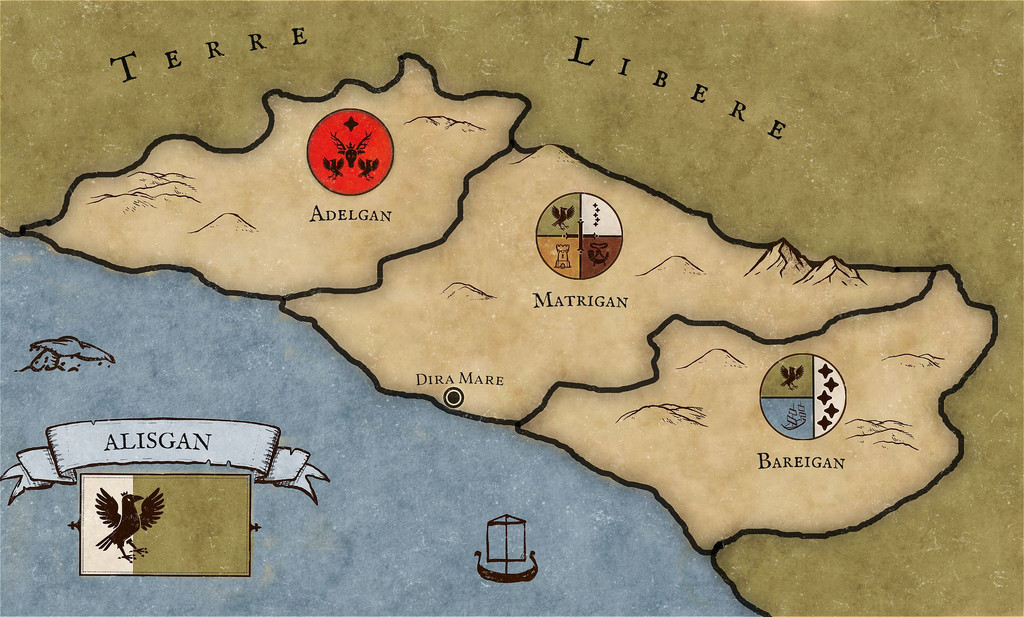
\includegraphics{alisei.jpg}
\caption{alisei.jpg}
\end{figure}

Il Regno degli Alisei è diviso in tre cantoni autonomi, ciascuno dei
quali amministrato da una delle tre tribù che compongono il popolo degli
Alisei. Il regno riflette un'armoniosa fusione di paesaggi distinti e un
patrimonio culturale condiviso. Il regno è diviso in tre cantoni
autonomi, ciascuno con una propria identità unica e amministrato da uno
dei 3 Clan di cui è composto il popolo degli Alisei:

\begin{itemize}
\tightlist
\item
  Adelgan: il Cantone Occidentale, patria del clan dei Adeli, gli ultimi
  a migrare nelle terre di Valtara.
\item
  Matrigan: il Cantone Centrale, patria del clan dei Matri e luogo in
  cui sorge la capitale del regno: Dira Mare.
\item
  Bareigan: il Cantone Orientale, patria del clan dei Bareni.
\end{itemize}

\subsubsection{Gli stemmi dei clan}\label{gli-stemmi-dei-clan}

Gli stemmi dei tre clan degli Alisei ci svelano molto della loro storia.
Tutti e tre gli stemmi incorporano simboli che richiamano la loro storia
di migrazione, che sono inoltre presenti nella bandiera nazionale.

Lo stemma del clan dei Matri si divide in quattro sezioni: in alto a
sinistra è raffigurato il corvo reale su uno sfondo verde. Il corvo
rappresenta l'animale che gli Alisei portavano con sé durante le loro
navigazioni, utilizzandolo come punto di riferimento per la terraferma.
Il verde dello sfondo simboleggia le fertili terre di Valtara dove
fecero sbarco. In alto a destra è rappresentata la costellazione
dell'arco, che costituiva il principale punto di riferimento per gli
Alisei durante le loro navigazioni. In basso a sinistra è raffigurata la
torre di guardia, simbolo della capitale situata nel cantone di questo
clan. In basso a destra è raffigurato il corno da battaglia su sfondo
rosso, simboleggiante le battaglie e il sangue versato prima della pace
e della fondazione del regno. Nello stemma dei Bareni è presente anche
il corvo reale e la costellazione dell'arco. In basso a destra è
raffigurata una nave, che commemora il periodo trascorso in mare durante
la migrazione e il viaggio degli Alisei.

Nello stemma del clan degli Adeli, è raffigurato l'animale simbolo del
clan, il cervo. Sotto di esso sono presenti due corvi reali, mentre in
alto è presente una stella, che simboleggia la costellazione dell'arco,
fondamentale per l'orientamento durante i viaggi e le navigazioni degli
Alisei.

\begin{figure}
\centering

\includegraphics{Screenshot_2023-10-20_170853.png}
\caption{I simboli ricorrenti in tutti gli stemmi}
\end{figure}

I simboli ricorrenti in tutti gli stemmi

\subsection{4. Demografia}\label{demografia}

\begin{center}\rule{0.5\linewidth}{0.5pt}\end{center}

La popolazione predominante è composta degli Alisei, una comunità umana
caratterizzata dal colore della pelle di un profondo tono di nero e gli
occhi di un verde brillante. Gli alisei, un tempo una delle minoranze
razziali più importanti della Rotrekia, sono oggi stanziati quasi
esclusivamente nella penisola Valtariana. La presenza significativa di
questa popolazione all'interno del regno costituisce l'elemento centrale
della tessitura sociale e culturale. Nonostante la varietà di razze e
gruppi etnici presenti, l'influenza degli Alisei si manifesta in ogni
aspetto della vita quotidiana, colorando le strade della capitale con le
loro tradizioni e le loro usanze. Nel regno, tuttavia, è presente
un'alta varietà di abitanti appartenenti ad ogni razza.

\subsection{5. Economia}\label{economia}

\begin{center}\rule{0.5\linewidth}{0.5pt}\end{center}

L'economia del Regno degli Alisei si basa su un sistema di mercato
aperto e in crescita, favorito da un clima di cooperazione e di libera
circolazione di persone e merci. Le attività commerciali prosperano
lungo le strade animate della capitale e dei centri urbani, con
un'attenzione particolare verso l'agricoltura, l'artigianato e il
commercio di beni esotici provenienti dalla Rotrekia. L'accento posto
sull'interconnessione e sul libero scambio ha favorito la formazione di
alleanze commerciali stabili sia all'interno del regno che con le terre
libere circostanti, promuovendo una crescita economica sostenibile e
inclusiva.

\subsection{6. Cultura}\label{cultura}

\begin{center}\rule{0.5\linewidth}{0.5pt}\end{center}

La cultura del Regno degli Alisei si evolve in un tessuto unico di
tradizioni, in cui gli usi secolari degli Alisei si intrecciano
armoniosamente con le radici culturali più ampie di Valtara. Nel corso
del tempo, le tradizioni e le celebrazioni degli Alisei si sono fusi con
elementi distintivi della cultura valtariana, dando vita a un panorama
culturale vibrante e dinamico che riflette l'unità e la diversità della
nazione. Le feste tradizionali degli Alisei si arricchiscono di elementi
valtariani, mentre le pratiche culinarie e gli stili artistici si
mescolano, creando un'esperienza culturale unica che è diventata una
parte fondamentale dell'identità culturale più ampia di Valtara. Questa
sinergia culturale ha contribuito a consolidare i legami tra le comunità
e a promuovere un senso di coesione nazionale basato sull'apprezzamento
reciproco e sul rispetto delle differenze culturali.

\subsection{7. Governo}\label{governo}

\begin{center}\rule{0.5\linewidth}{0.5pt}\end{center}

Il Regno degli Alisei adotta un sistema di governo basato su una
monarchia costituzionale, in cui il sovrano agisce come figura di
rappresentanza e di unità nazionale, mentre il potere legislativo è
affidato a un parlamento eletto democraticamente. La costituzione
stabilisce i diritti e le responsabilità dei cittadini, garantendo
l'uguaglianza di fronte alla legge e la protezione dei diritti umani
fondamentali. Le decisioni cruciali sono prese in consultazione con gli
organi rappresentativi e con l'approvazione del popolo, promuovendo una
governance trasparente e responsabile che tiene conto dei valori di
giustizia e di equità.
